\documentclass[12pt,a4paper]{article}

% ── PACKAGES ──
\usepackage[utf8]{inputenc}
\usepackage[T1]{fontenc}
\usepackage[french]{babel}
\usepackage{geometry}
\usepackage{graphicx}
\usepackage{booktabs}
\usepackage{tabularx}
\usepackage{longtable}
\usepackage{array}
\usepackage{xcolor}
\usepackage{colortbl}
\usepackage{hyperref}
\usepackage{fancyhdr}
\usepackage{titlesec}
\usepackage{enumitem}
\usepackage{tcolorbox}
\usepackage{pdfpages}
\usepackage{float}
\usepackage{setspace}
\usepackage{parskip}
\usepackage{lmodern}

% ── PAGE GEOMETRY ──
\geometry{
  a4paper,
  top=2.5cm, bottom=2.5cm,
  left=2.5cm, right=2.5cm
}

% ── COULEURS ──
\definecolor{primaryblue}{HTML}{3B82F6}
\definecolor{darkblue}{HTML}{1E3A5F}
\definecolor{lightblue}{HTML}{EFF6FF}
\definecolor{accentpurple}{HTML}{8B5CF6}
\definecolor{successgreen}{HTML}{10B981}
\definecolor{warningorange}{HTML}{F59E0B}
\definecolor{dangered}{HTML}{EF4444}
\definecolor{darkgray}{HTML}{374151}
\definecolor{lightgray}{HTML}{F9FAFB}
\definecolor{bordergray}{HTML}{E5E7EB}
\definecolor{textmuted}{HTML}{6B7280}

% ── HYPERLINKS ──
\hypersetup{
  colorlinks=true,
  linkcolor=primaryblue,
  urlcolor=primaryblue,
  citecolor=primaryblue,
  pdftitle={Cahier des Charges - UML-to-Code v2},
  pdfauthor={Abakar Mahamat Brahim},
  pdfsubject={Mini-Projet Soutenance GL3 INSTA 2026}
}

% ── TITRES ──
\titleformat{\section}
  {\large\bfseries\color{darkblue}}
  {\thesection.}{0.8em}{}
  [\vspace{-0.3em}\textcolor{primaryblue}{\rule{\linewidth}{1.5pt}}]

\titleformat{\subsection}
  {\normalsize\bfseries\color{darkblue}}
  {\thesubsection}{0.8em}{}

\titleformat{\subsubsection}
  {\normalsize\bfseries\color{darkgray}}
  {\thesubsubsection}{0.8em}{}

% ── EN-TÊTES / PIEDS DE PAGE ──
\setlength{\headheight}{24pt}
\addtolength{\topmargin}{-12pt}
\pagestyle{fancy}
\fancyhf{}
\fancyhead[L]{\small\textcolor{textmuted}{CDC — UML-to-Code v2.0 \textbar\ INSTA Abéché 2026}}
\fancyhead[R]{\small\textcolor{textmuted}{Abakar — GL3}}
\fancyfoot[C]{\small\textcolor{textmuted}{\thepage}}
\renewcommand{\headrulewidth}{0.4pt}
\renewcommand{\footrulewidth}{0pt}
\renewcommand{\headrule}{\hbox to\headwidth{\color{bordergray}\leaders\hrule height \headrulewidth\hfill}}

% ── TCOLORBOX STYLES ──
\tcbuselibrary{skins, breakable}
\newtcolorbox{infobox}[1][]{
  colback=lightblue, colframe=primaryblue,
  boxrule=0.8pt, arc=6pt,
  left=8pt, right=8pt, top=6pt, bottom=6pt,
  #1
}
\newtcolorbox{successbox}[1][]{
  colback=green!5, colframe=successgreen,
  boxrule=0.8pt, arc=6pt,
  left=8pt, right=8pt, top=6pt, bottom=6pt,
  #1
}

% ── COMMANDES UTILES ──
\newcommand{\badge}[2]{%
  \colorbox{#1!15}{\textcolor{#1}{\small\textbf{#2}}}%
}
\newcommand{\highpriority}{\badge{dangered}{Haute}}
\newcommand{\mediumpriority}{\badge{warningorange}{Moyenne}}
\newcommand{\lowpriority}{\badge{successgreen}{Basse}}

% ─────────────────────────────────────────────
\begin{document}
\setstretch{1.15}

% ── PAGE DE GARDE (PDF externe) ──

\includepdf[pages=1]{PageGarde_CDC.pdf}

% ── TABLE DES MATIÈRES ──
\tableofcontents
\newpage

% ─────────────────────────────────────────────
\section{Introduction}

\subsection{Contexte général}

Dans le domaine du Génie Logiciel, la modélisation UML (\textit{Unified Modeling Language}) constitue une étape fondamentale du cycle de développement. Elle permet de concevoir et de documenter l'architecture d'un système avant son implémentation. Cependant, le passage du modèle conceptuel au code source reste une tâche manuelle, répétitive et source d'erreurs.

Ce projet s'inscrit dans le paradigme du \textbf{Développement Dirigé par les Modèles} (MDD — \textit{Model-Driven Development}), qui préconise la génération automatique de code à partir de modèles de haut niveau. L'intégration de l'Intelligence Artificielle générative dans ce processus représente une avancée significative, permettant de produire un code plus complet, contextuel et directement exploitable.

\subsection{Présentation du projet}

Le projet \textbf{« UML-to-Code »} vise à développer une application web full-stack permettant de transformer automatiquement un diagramme de classes UML en code source fonctionnel, en exploitant le modèle d'IA générative \textbf{Groq Llama 3.3-70b}. L'utilisateur soumet un diagramme (au format XMI, image ou PDF), et l'application génère le code Python ou PHP correspondant, ainsi qu'un serveur Flask complet et opérationnel, le tout exportable en archive ZIP.

\begin{infobox}
  \textbf{Changement majeur (v1 $\rightarrow$ v2) :} Le moteur d'IA a été migré de \textit{Google Gemma via API Gemini} vers \textbf{Groq Llama 3.3-70b (API Groq)}, offrant des temps de génération réduits (~2 secondes) et un code de meilleure qualité. L'interface a également été entièrement enrichie.
\end{infobox}

\subsection{Objectifs du document}

Ce Cahier des Charges a pour objectifs de :
\begin{itemize}[leftmargin=1.5em]
  \item Définir le périmètre fonctionnel et technique du projet
  \item Identifier les acteurs et leurs interactions avec le système
  \item Spécifier les exigences fonctionnelles et non fonctionnelles
  \item Présenter l'architecture technique retenue
  \item Établir le planning de réalisation
  \item Définir les critères d'acceptation et les livrables attendus
\end{itemize}

% ─────────────────────────────────────────────
\section{Analyse de l'Existant}

\subsection{Outils existants}

Plusieurs outils de transformation UML vers code existent sur le marché. Une analyse comparative permet d'identifier leurs limites :

\begin{table}[H]
\centering
\renewcommand{\arraystretch}{1.3}
\begin{tabularx}{\textwidth}{|l|l|l|X|}
\hline
\rowcolor{darkblue!90}
\textcolor{white}{\textbf{Outil}} &
\textcolor{white}{\textbf{Langages générés}} &
\textcolor{white}{\textbf{Format entrée}} &
\textcolor{white}{\textbf{Limites principales}} \\
\hline
Acceleo (Eclipse) & Java, Python, PHP & XMI/EMF & Très complexe, lourd à installer \\
\hline
\rowcolor{lightgray}
AndroMDA & Java EE uniquement & XMI & Limité à Java, pas d'IA \\
\hline
GenMyModel & Java, Python & En ligne & Payant, pas open source \\
\hline
\rowcolor{lightgray}
StarUML Plugins & JavaScript, Java & .mdj & Limité, pas d'IA générative \\
\hline
Solutions manuelles & Tous langages & Tous formats & Lent, source d'erreurs \\
\hline
\end{tabularx}
\caption{Comparatif des outils existants de transformation UML vers code}
\end{table}

\subsection{Valeur ajoutée du projet}

Par rapport aux solutions existantes, UML-to-Code apporte :
\begin{itemize}[leftmargin=1.5em]
  \item Intégration d'une IA générative (\textbf{Groq Llama 3.3-70b}) pour un code contextuel et complet
  \item Support de plusieurs formats d'entrée : XMI, image PNG/JPG, PDF
  \item Génération automatique d'un serveur Flask complet et opérationnel
  \item Interface web moderne avec design \textbf{Glassmorphism}, thème sombre/clair
  \item Éditeur de code intégré (\textbf{Monaco Editor} — le moteur de VS Code)
  \item Gestion de l'historique local des 10 dernières générations
  \item Export en archive ZIP (code + serveur Flask)
  \item Solution légère, open source et sans installation complexe
\end{itemize}

% ─────────────────────────────────────────────
\section{Périmètre du Projet}

\subsection{Ce qui est inclus}

\begin{itemize}[leftmargin=1.5em]
  \item Acceptation de diagrammes UML au format XMI (StarUML)
  \item Acceptation de diagrammes sous forme d'image (PNG, JPG)
  \item Acceptation de diagrammes intégrés dans un fichier PDF
  \item Génération de code Python (classes, attributs, méthodes, héritage)
  \item Génération de code PHP (classes avec visibilité, constructeur)
  \item Génération automatique d'un serveur Flask Python complet avec routes CRUD
  \item Interface web React.js (Glassmorphism) avec upload, visualisation et téléchargement
  \item Intégration de \textbf{Monaco Editor} pour la lecture et l'édition du code généré
  \item Système d'historique local (localStorage) — 10 dernières générations
  \item Mode sombre / mode clair (bascule dynamique)
  \item Barre de progression en temps réel avec étapes détaillées
  \item Aperçu visuel du diagramme uploadé (pour PNG/JPG)
  \item Statistiques de génération : lignes, classes, méthodes, temps
  \item Notifications toast (feedback utilisateur)
  \item Export ZIP du projet complet (code + serveur Flask)
  \item Copie du code généré en un clic
  \item Téléchargement du code généré en fichier \texttt{.py} ou \texttt{.php}
  \item Navbar responsive avec menu hamburger mobile
\end{itemize}

\subsection{Ce qui est exclu}

\begin{itemize}[leftmargin=1.5em]
  \item Les diagrammes de séquence, d'activité ou de cas d'utilisation
  \item La génération de bases de données ou de requêtes SQL
  \item La génération de code Java (hors scope pour ce projet)
  \item L'hébergement en ligne de l'application (démo locale uniquement)
  \item L'authentification et la gestion multi-utilisateurs centralisée
  \item La sauvegarde serveur (historique en localStorage uniquement)
\end{itemize}

% ─────────────────────────────────────────────
\section{Acteurs et Cas d'Utilisation}

\subsection{Acteurs identifiés}

\begin{table}[H]
\centering
\renewcommand{\arraystretch}{1.3}
\begin{tabularx}{\textwidth}{|l|l|X|}
\hline
\rowcolor{darkblue!90}
\textcolor{white}{\textbf{Acteur}} &
\textcolor{white}{\textbf{Rôle}} &
\textcolor{white}{\textbf{Interactions principales}} \\
\hline
\textbf{Utilisateur} & Étudiant ou développeur & Upload fichier, choix options, génération, visualisation Monaco Editor, copie/téléchargement, consultation historique, bascule thème \\
\hline
\rowcolor{lightgray}
\textbf{API Groq (IA)} & Modèle Llama 3.3-70b & Reçoit la description UML extraite, retourne le code généré \\
\hline
\textbf{Backend Flask} & Serveur Python & Orchestration, parsing XMI/image/PDF, appel API Groq, génération ZIP \\
\hline
\rowcolor{lightgray}
\textbf{localStorage} & Stockage navigateur & Persiste l'historique des 10 dernières générations et le thème \\
\hline
\end{tabularx}
\caption{Acteurs du système UML-to-Code}
\end{table}

\subsection{Cas d'utilisation principaux}

\begin{enumerate}[leftmargin=1.5em]
  \item L'utilisateur uploade un fichier XMI, image PNG/JPG ou PDF (drag-and-drop ou clic)
  \item Si image PNG/JPG : le système affiche un aperçu visuel du diagramme
  \item L'utilisateur choisit le langage cible (Python ou PHP) et le mode (Algorithmique ou IA Groq)
  \item La barre de progression affiche les étapes en temps réel
  \item Le système détecte le format, parse le diagramme et envoie à Groq si mode IA
  \item Le code généré s'affiche dans le Monaco Editor (onglet Code + onglet Serveur Flask)
  \item Les statistiques de génération sont affichées (lignes, classes, temps)
  \item L'utilisateur copie, télécharge en \texttt{.py}/\texttt{.php}, ou exporte en ZIP
  \item La génération est sauvegardée dans l'historique local (max 10 entrées)
  \item L'utilisateur peut consulter et recharger ses anciennes générations via l'historique
\end{enumerate}

\subsection{Diagramme de Cas d'Utilisation}

\begin{figure}[H]
  \centering
  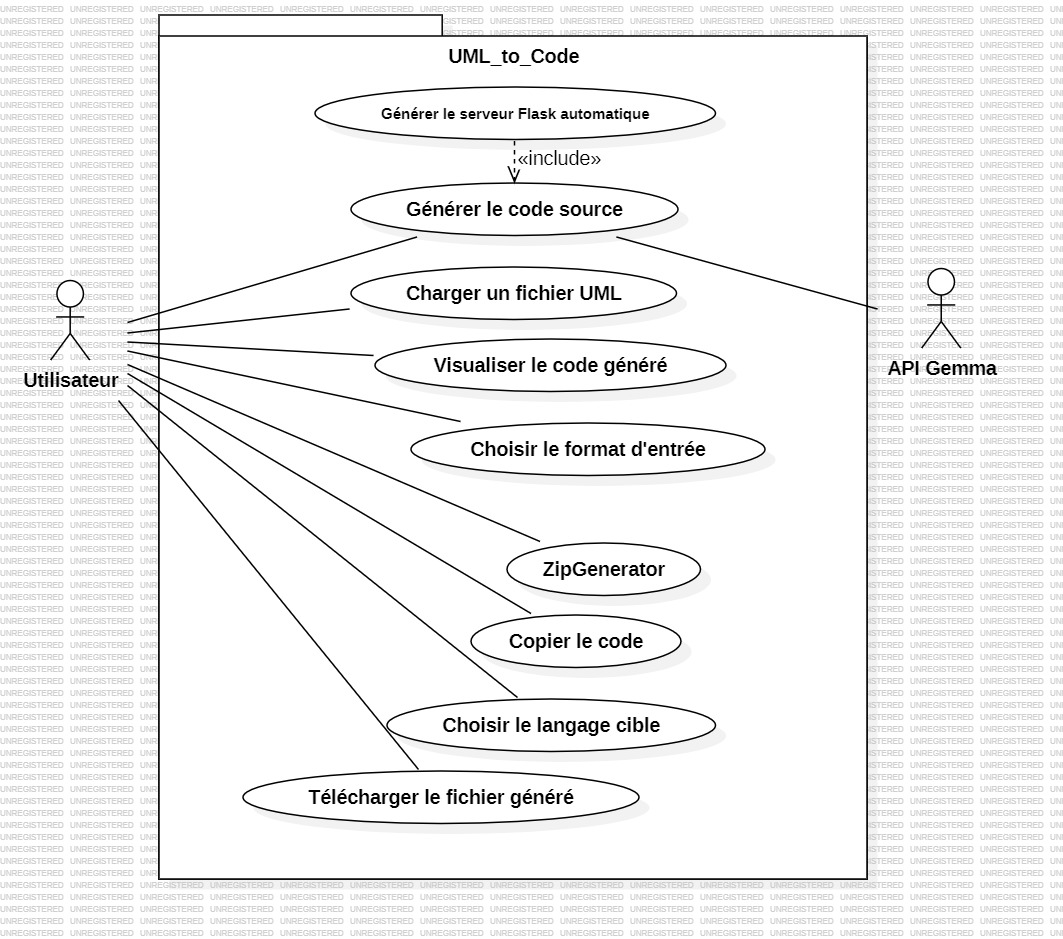
\includegraphics[width=0.85\textwidth]{UCD_UML_to_Code.jpg}
  \caption{Diagramme de cas d'utilisation — UML-to-Code}
\end{figure}

% ─────────────────────────────────────────────
\section{Exigences Fonctionnelles}

\subsection{Module Upload}

\begin{table}[H]
\centering
\renewcommand{\arraystretch}{1.3}
\begin{tabularx}{\textwidth}{|c|X|c|}
\hline
\rowcolor{darkblue!90}
\textcolor{white}{\textbf{ID}} &
\textcolor{white}{\textbf{Exigence}} &
\textcolor{white}{\textbf{Priorité}} \\
\hline
EF-01 & Accepter les fichiers XMI exportés depuis StarUML & \highpriority \\
\hline
\rowcolor{lightgray}
EF-02 & Accepter les images PNG et JPG de diagrammes UML & \highpriority \\
\hline
EF-03 & Accepter les fichiers PDF contenant un diagramme UML & \mediumpriority \\
\hline
\rowcolor{lightgray}
EF-04 & Valider le format du fichier avant traitement & \highpriority \\
\hline
EF-05 & Afficher un message d'erreur en cas de format invalide & \highpriority \\
\hline
\rowcolor{lightgray}
EF-06 & Afficher un aperçu visuel du diagramme pour PNG/JPG & \mediumpriority \\
\hline
EF-07 & Permettre la suppression du fichier sélectionné avant génération & \mediumpriority \\
\hline
\end{tabularx}
\caption{Exigences fonctionnelles — Module Upload}
\end{table}

\subsection{Module Parsing}

\begin{table}[H]
\centering
\renewcommand{\arraystretch}{1.3}
\begin{tabularx}{\textwidth}{|c|X|c|}
\hline
\rowcolor{darkblue!90}
\textcolor{white}{\textbf{ID}} &
\textcolor{white}{\textbf{Exigence}} &
\textcolor{white}{\textbf{Priorité}} \\
\hline
EF-08 & Parser les classes, attributs et méthodes depuis un XMI & \highpriority \\
\hline
\rowcolor{lightgray}
EF-09 & Extraire les relations d'héritage entre classes & \highpriority \\
\hline
EF-10 & Extraire les associations et agrégations & \mediumpriority \\
\hline
\rowcolor{lightgray}
EF-11 & Envoyer l'image/PDF directement à Groq (vision IA) & \highpriority \\
\hline
\end{tabularx}
\caption{Exigences fonctionnelles — Module Parsing}
\end{table}

\subsection{Module Génération IA}

\begin{table}[H]
\centering
\renewcommand{\arraystretch}{1.3}
\begin{tabularx}{\textwidth}{|c|X|c|}
\hline
\rowcolor{darkblue!90}
\textcolor{white}{\textbf{ID}} &
\textcolor{white}{\textbf{Exigence}} &
\textcolor{white}{\textbf{Priorité}} \\
\hline
EF-12 & Appeler l'API Groq (Llama 3.3-70b) avec la description UML extraite & \highpriority \\
\hline
\rowcolor{lightgray}
EF-13 & Générer le code Python complet avec \texttt{\_\_init\_\_}, getters, setters & \highpriority \\
\hline
EF-14 & Générer le code PHP avec visibilité, constructeur, getters & \highpriority \\
\hline
\rowcolor{lightgray}
EF-15 & Générer un serveur Flask automatique avec les routes CRUD & \highpriority \\
\hline
EF-16 & Permettre le choix du langage cible : Python ou PHP & \highpriority \\
\hline
\rowcolor{lightgray}
EF-17 & Permettre le choix du mode : Algorithmique (XMI) ou IA Groq & \highpriority \\
\hline
EF-18 & Afficher les statistiques de génération (lignes, classes, méthodes, temps) & \mediumpriority \\
\hline
\end{tabularx}
\caption{Exigences fonctionnelles — Module Génération IA}
\end{table}

\subsection{Module Interface et Expérience Utilisateur}

\begin{table}[H]
\centering
\renewcommand{\arraystretch}{1.3}
\begin{tabularx}{\textwidth}{|c|X|c|}
\hline
\rowcolor{darkblue!90}
\textcolor{white}{\textbf{ID}} &
\textcolor{white}{\textbf{Exigence}} &
\textcolor{white}{\textbf{Priorité}} \\
\hline
EF-19 & Afficher le code généré dans Monaco Editor (VS Code intégré) & \highpriority \\
\hline
\rowcolor{lightgray}
EF-20 & Afficher onglet Code et onglet Serveur Flask séparément & \highpriority \\
\hline
EF-21 & Permettre la copie du code en un clic & \highpriority \\
\hline
\rowcolor{lightgray}
EF-22 & Permettre le téléchargement du fichier \texttt{.py} ou \texttt{.php} & \highpriority \\
\hline
EF-23 & Permettre l'export en archive ZIP (code + serveur Flask) & \highpriority \\
\hline
\rowcolor{lightgray}
EF-24 & Afficher une barre de progression avec étapes détaillées en temps réel & \highpriority \\
\hline
EF-25 & Implémenter un historique local (localStorage) des 10 dernières générations & \highpriority \\
\hline
\rowcolor{lightgray}
EF-26 & Permettre de recharger une génération passée depuis l'historique & \highpriority \\
\hline
EF-27 & Permettre d'effacer l'historique local & \mediumpriority \\
\hline
\rowcolor{lightgray}
EF-28 & Fournir une interface premium type ``Glassmorphism'' & \mediumpriority \\
\hline
EF-29 & Implémenter le mode sombre / mode clair (persisté en localStorage) & \mediumpriority \\
\hline
\rowcolor{lightgray}
EF-30 & Afficher des notifications toast (succès, erreur, info) & \mediumpriority \\
\hline
EF-31 & Navbar responsive avec menu hamburger pour mobile & \mediumpriority \\
\hline
\rowcolor{lightgray}
EF-32 & Animations et transitions modernes (fadeIn, float, slideUp) & \lowpriority \\
\hline
\end{tabularx}
\caption{Exigences fonctionnelles — Module Interface UX}
\end{table}

% ─────────────────────────────────────────────
\section{Exigences Non Fonctionnelles}

\begin{table}[H]
\centering
\renewcommand{\arraystretch}{1.3}
\begin{tabularx}{\textwidth}{|l|X|X|}
\hline
\rowcolor{darkblue!90}
\textcolor{white}{\textbf{Catégorie}} &
\textcolor{white}{\textbf{Exigence}} &
\textcolor{white}{\textbf{Critère mesurable}} \\
\hline
\textbf{Performance} & Temps de réponse de la génération & $<$ 15 secondes par diagramme \\
\hline
\rowcolor{lightgray}
\textbf{Disponibilité} & Fonctionne en local & Sans connexion (sauf API Groq) \\
\hline
\textbf{Fiabilité} & Taux de succès de la génération & $>$ 90\% sur les cas de test \\
\hline
\rowcolor{lightgray}
\textbf{Maintenabilité} & Code source documenté et structuré & Commentaires sur chaque fonction \\
\hline
\textbf{Portabilité} & Fonctionne sur Windows et Linux & Testé sur les deux systèmes \\
\hline
\rowcolor{lightgray}
\textbf{Sécurité} & Clé API stockée en variable d'environnement & Fichier \texttt{.env} non versionné (gitignore) \\
\hline
\textbf{Utilisabilité} & Interface intuitive sans formation & Prise en main $<$ 5 minutes \\
\hline
\rowcolor{lightgray}
\textbf{Responsivité} & Interface adaptée mobile et desktop & Testé sur écrans 320px à 1440px \\
\hline
\end{tabularx}
\caption{Exigences non fonctionnelles}
\end{table}






% ─────────────────────────────────────────────
\newpage
\section{Architecture Technique}

\subsection{Stack technologique}

\begin{table}[H]
\centering
\renewcommand{\arraystretch}{1.3}
\begin{tabularx}{\textwidth}{|l|l|l|X|}
\hline
\rowcolor{darkblue!90}
\textcolor{white}{\textbf{Couche}} &
\textcolor{white}{\textbf{Technologie}} &
\textcolor{white}{\textbf{Version}} &
\textcolor{white}{\textbf{Rôle}} \\
\hline
Frontend & React.js + Vite & 6.x & Interface utilisateur web \\
\hline
\rowcolor{lightgray}
Éditeur & Monaco Editor & Latest & Éditeur de code intégré (VS Code) \\
\hline
Icônes & React Icons & Latest & Icônes UI (FaHome, FaBolt, etc.) \\
\hline
\rowcolor{lightgray}
HTTP Client & Axios & Latest & Requêtes Frontend $\rightarrow$ Backend \\
\hline
Backend & Python Flask & 3.0.0 & Serveur API REST \\
\hline
\rowcolor{lightgray}
IA & Groq Llama 3.3-70b & Latest & Génération de code intelligent \\
\hline
Parsing XMI & xml.etree & Natif Python & Extraction classes UML depuis XMI \\
\hline
\rowcolor{lightgray}
Parsing Image & PyMuPDF & 1.27 & Conversion PDF $\rightarrow$ image \\
\hline
Export & zipfile & Natif Python & Export projet ZIP \\
\hline
\rowcolor{lightgray}
Stockage & localStorage & Natif Web & Historique local + thème \\
\hline
Versioning & Git + GitHub & — & Gestion du code source \\
\hline
\end{tabularx}
\caption{Stack technologique du projet}
\end{table}

\subsection{Architecture globale}

Le système suit une architecture client-serveur en 3 couches :

\begin{enumerate}[leftmargin=1.5em]
  \item \textbf{Couche Présentation} : React.js — interface Glassmorphism, Monaco Editor, historique localStorage, thème sombre/clair, animations
  \item \textbf{Couche Métier} : Flask Python — orchestration, parsing XMI/image/PDF, appel API Groq, génération ZIP
  \item \textbf{Couche IA} : API Groq (Llama 3.3-70b) — génération intelligente du code Python/PHP/Flask
\end{enumerate}

\begin{center}
\renewcommand{\arraystretch}{1.4}
\begin{tabular}{c}
  \begin{tcolorbox}[
    colback=primaryblue!10, colframe=primaryblue,
    arc=6pt, boxrule=1pt,
    width=0.75\textwidth,
    halign=center
  ]
    \textbf{FRONTEND} (React + Vite)\\
    \small Monaco Editor \textbullet\ Toast \textbullet\ Historique \textbullet\ Thèmes
  \end{tcolorbox}\\[-2pt]
  {\color{primaryblue}\large $\downarrow$} \quad \textit{\small HTTP REST (axios)} \quad {\color{primaryblue}\large $\downarrow$}\\[-2pt]
  \begin{tcolorbox}[
    colback=accentpurple!10, colframe=accentpurple,
    arc=6pt, boxrule=1pt,
    width=0.75\textwidth,
    halign=center
  ]
    \textbf{BACKEND} (Python Flask)\\
    \small Parser XMI \textbullet\ Orchestration \textbullet\ Routes API \textbullet\ ZIP
  \end{tcolorbox}\\[-2pt]
  {\color{accentpurple}\large $\downarrow$} \quad \textit{\small API Call} \quad {\color{accentpurple}\large $\downarrow$}\\[-2pt]
  \begin{tcolorbox}[
    colback=successgreen!10, colframe=successgreen,
    arc=6pt, boxrule=1pt,
    width=0.75\textwidth,
    halign=center
  ]
    \textbf{IA} --- Groq Llama 3.3-70b\\
    \small Génération code Python \textbullet\ PHP \textbullet\ Flask
  \end{tcolorbox}
\end{tabular}
\end{center}

\subsection{Diagramme de Classes}

\begin{figure}[H]
  \centering
  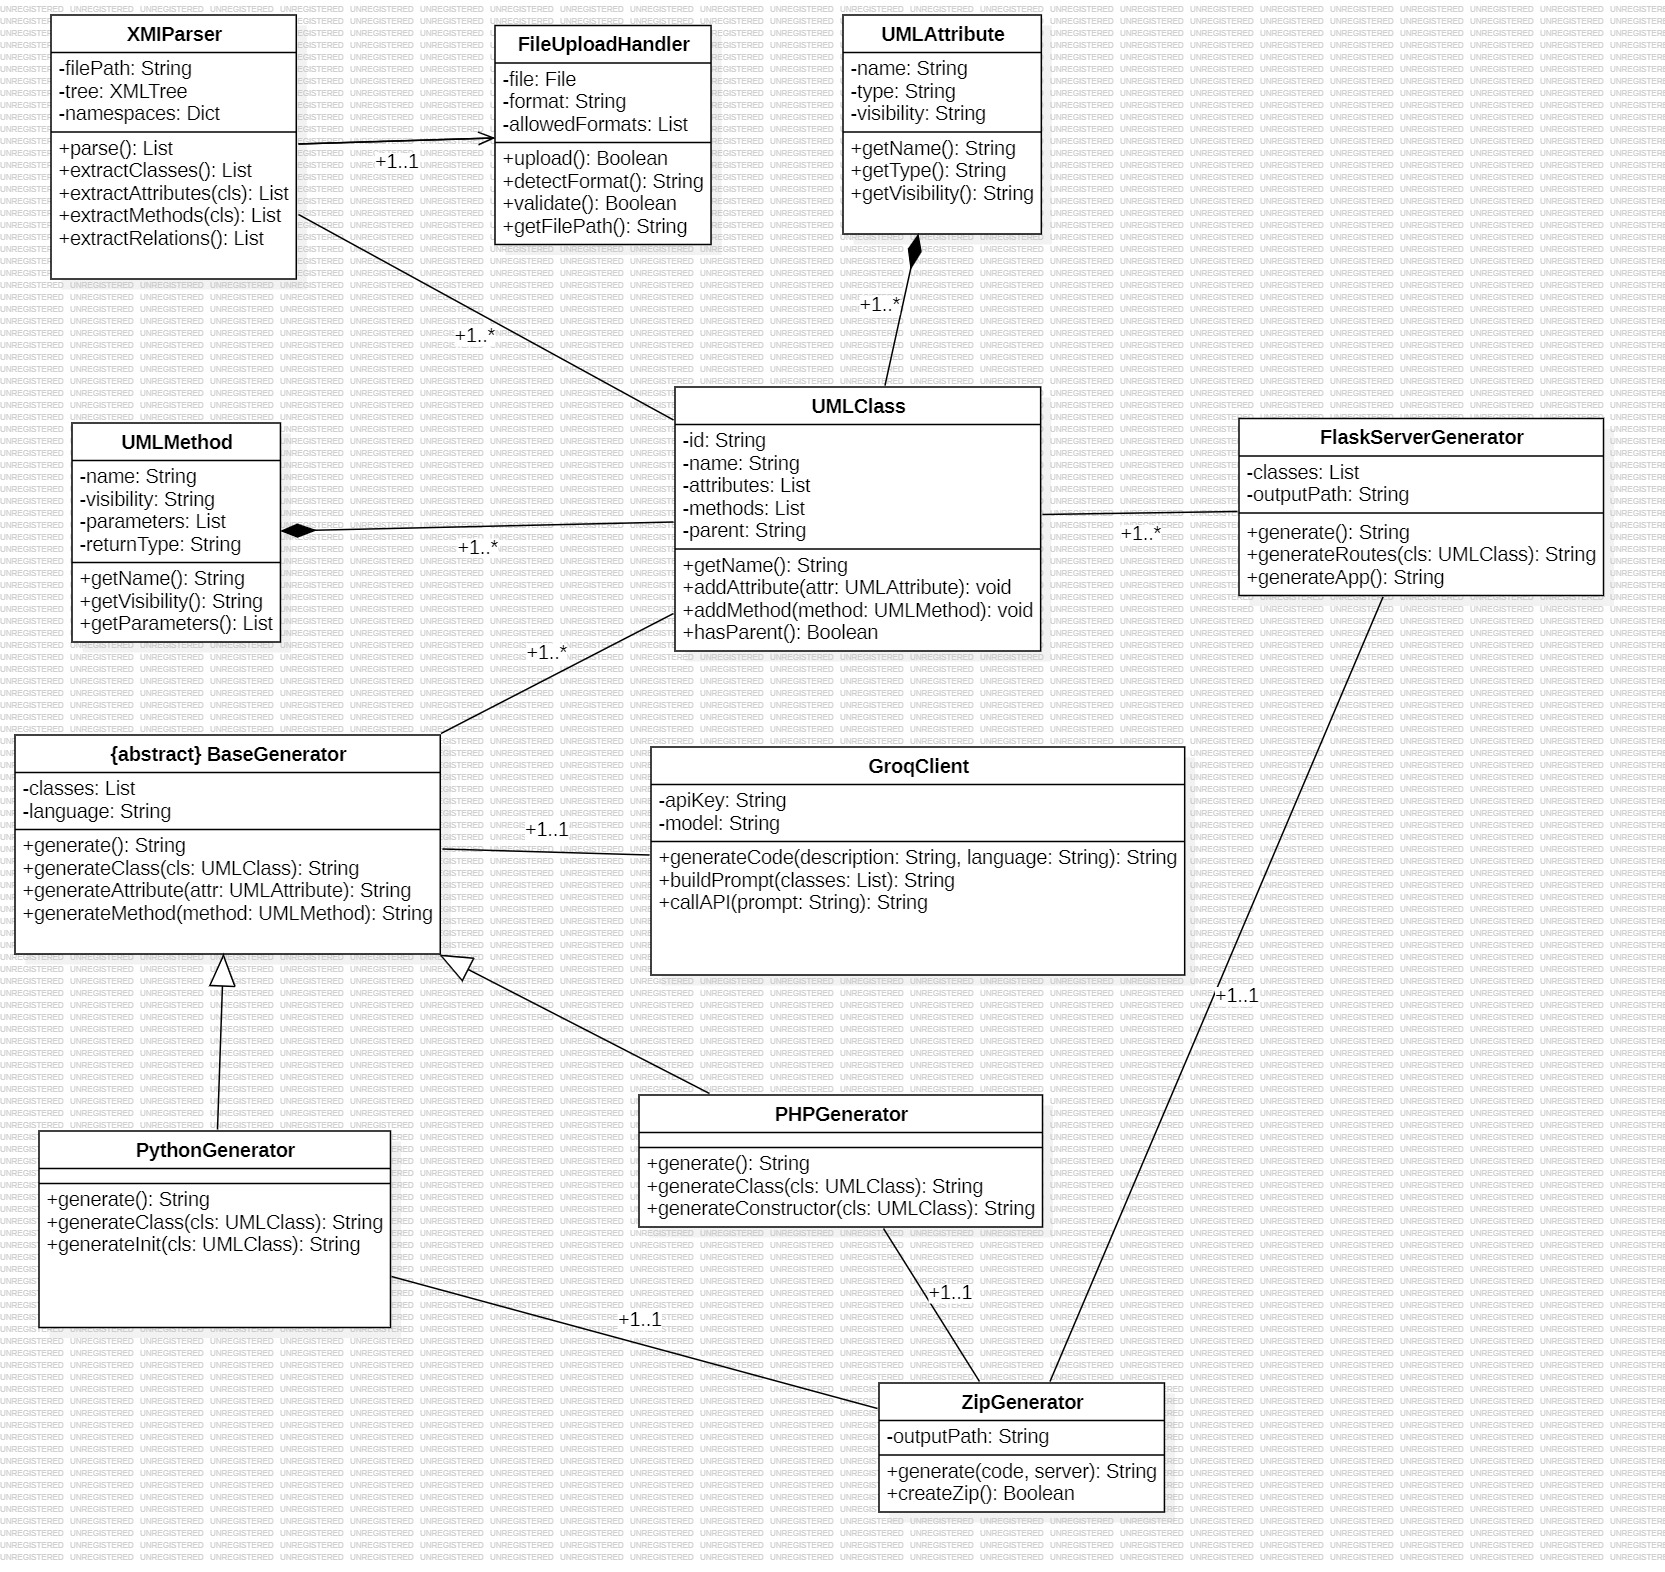
\includegraphics[width=\textwidth]{CD_UML_to_Code.jpg}
  \caption{Diagramme de classes — UML-to-Code}
\end{figure}

\subsection{Diagramme de Séquence}

\begin{figure}[H]
  \centering
  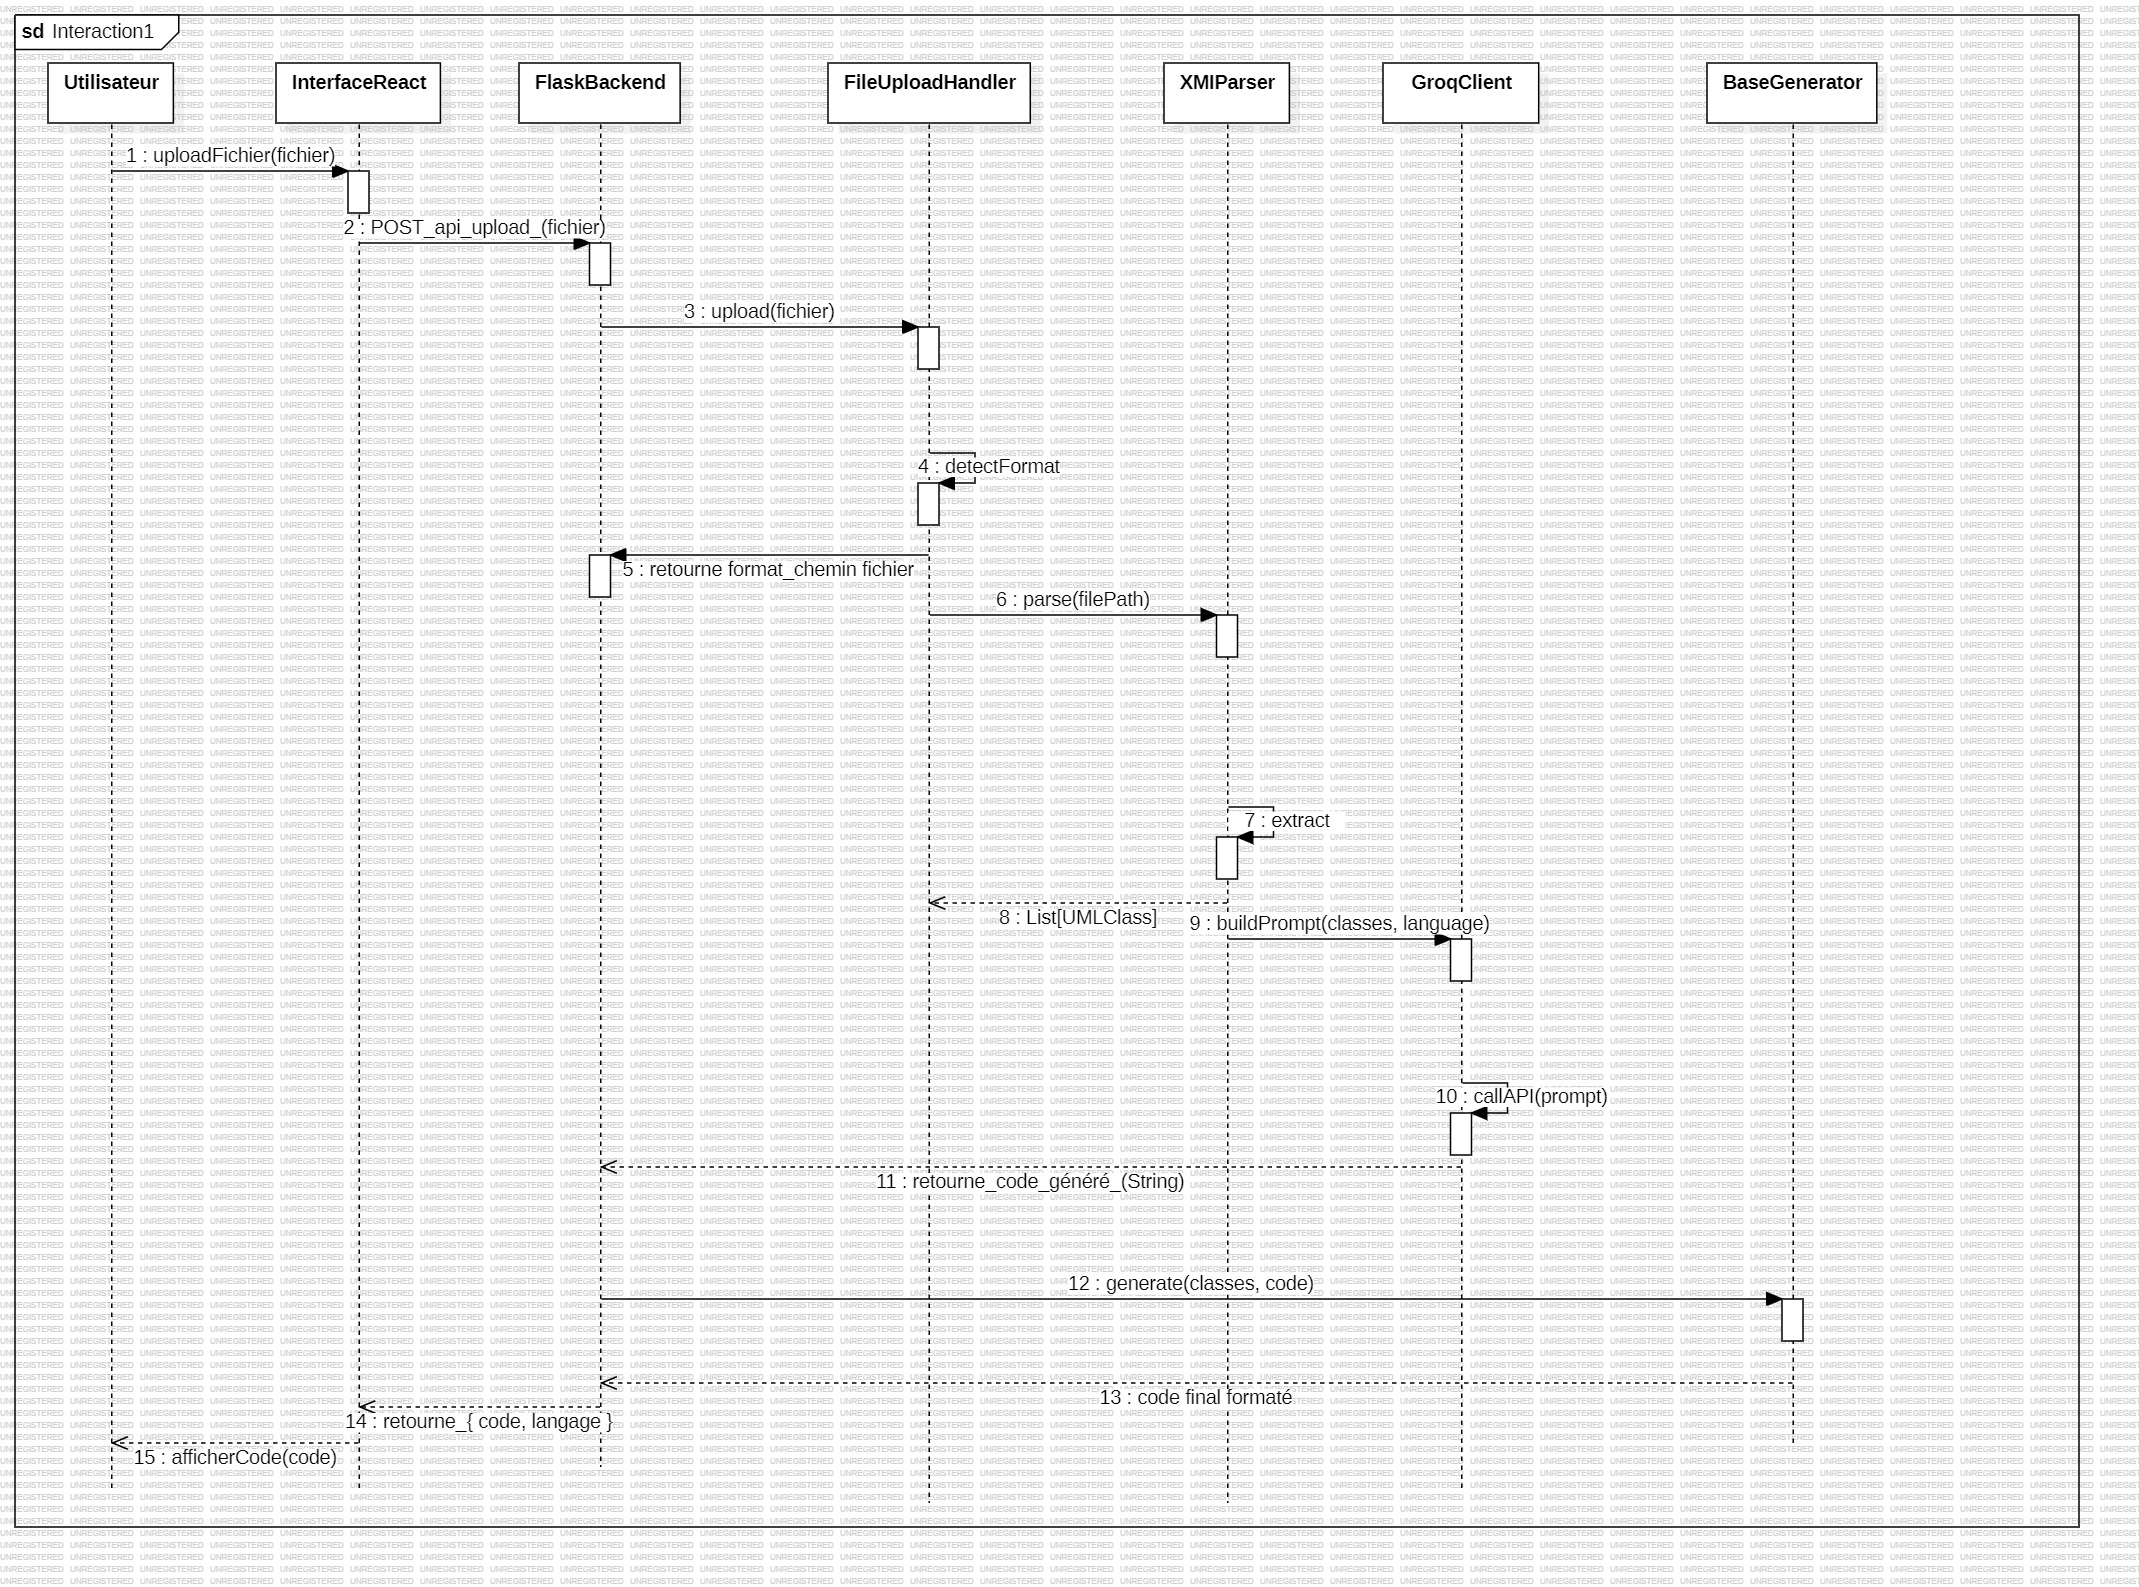
\includegraphics[width=\textwidth]{SD_Generation_Code.jpg}
  \caption{Diagramme de séquence — Génération de code}
\end{figure}

\subsection{Structure des dossiers}

\begin{tcolorbox}[colback=gray!5, colframe=bordergray, arc=6pt]
\small\ttfamily
\begin{tabbing}
uml-to-code/ \\
\quad \= backend/ \quad \= \kill
\> backend/                        \> \# Serveur Python Flask \\
\> \quad app.py                    \> \# Point d'entrée Flask \\
\> \quad routes/upload.py          \> \# Endpoints API \\
\> \quad parser/xmi\_parser.py     \> \# Parsing fichiers XMI \\
\> \quad parser/image\_parser.py   \> \# Analyse image/PDF via IA \\
\> \quad ai/gemma\_client.py       \> \# Client API Groq \\
\> \quad generator/python\_generator.py \> \# Générateur Python \\
\> \quad generator/php\_generator.py    \> \# Générateur PHP \\
\> \quad generator/server\_generator.py \> \# Générateur Flask \\
\> \quad generator/zip\_generator.py    \> \# Export ZIP \\
\> frontend/                       \> \# Interface React + Vite \\
\> \quad src/App.jsx                \> \# Composant principal \\
\> \quad src/App.css                \> \# Styles complets \\
\> examples/test.xmi               \> \# Fichier XMI de test \\
\> .gitignore \\
\> README.md \\
\end{tabbing}
\end{tcolorbox}

% ─────────────────────────────────────────────
\section{Cycle de Vie du Projet}

\subsection{Choix du cycle de vie : Modèle Incrémental}

Le modèle de cycle de vie retenu pour ce projet est le \textbf{modèle incrémental}. Ce choix est motivé par trois raisons principales :
\begin{itemize}[leftmargin=1.5em]
  \item La durée courte du projet (3 semaines) nécessite des livraisons rapides et concrètes
  \item Le projet est réalisé en solo, ce qui exclut les cycles nécessitant une équipe (Scrum)
  \item L'intégration d'une IA générative (Groq) introduit des incertitudes techniques qui imposent un ajustement progressif
\end{itemize}

\subsection{Comparaison des cycles de vie}

\begin{table}[H]
\centering
\renewcommand{\arraystretch}{1.3}
\begin{tabular}{|l|c|c|c|l|}
\hline
\rowcolor{darkblue!90}
\textcolor{white}{\textbf{Cycle de vie}} &
\textcolor{white}{\textbf{Durée idéale}} &
\textcolor{white}{\textbf{Solo}} &
\textcolor{white}{\textbf{3 semaines}} &
\textcolor{white}{\textbf{Décision}} \\
\hline
Cascade (Waterfall) & 6+ mois & Oui & Non & \badge{dangered}{Rejeté} \\
\hline
\rowcolor{lightgray}
Cycle en V & 3+ mois & Oui & Limite & \badge{dangered}{Rejeté} \\
\hline
Agile / Scrum & Continu & Limite & Oui & \badge{dangered}{Rejeté} \\
\hline
\rowcolor{lightgray}
\textbf{Incrémental} & 1–6 mois & Oui & Oui & \badge{successgreen}{RETENU} \\
\hline
\end{tabular}
\caption{Comparaison des cycles de vie}
\end{table}

\subsection{Les 5 incréments du projet}

\begin{table}[H]
\centering
\renewcommand{\arraystretch}{1.3}
\begin{tabularx}{\textwidth}{|c|l|X|c|}
\hline
\rowcolor{darkblue!90}
\textcolor{white}{\textbf{Incrément}} &
\textcolor{white}{\textbf{Période}} &
\textcolor{white}{\textbf{Fonctionnalités ajoutées}} &
\textcolor{white}{\textbf{Version}} \\
\hline
\textbf{0 — Préparation} & 05–07 mai & Questions prof, étude XMI, recherche, CDC & v0.0 \\
\hline
\rowcolor{lightgray}
\textbf{1 — Fondations} & 08–14 mai & Architecture, parser XMI, modèle de données, test API Groq & v0.1 \\
\hline
\textbf{2 — Cœur IA \& UI} & 15–21 mai & Groq complet, générateurs Python+PHP, Flask auto, React Glassmorphism, Monaco Editor, Historique local & v0.2 \\
\hline
\rowcolor{lightgray}
\textbf{3 — Finalisation} & 22–26 mai & Tests, corrections, export ZIP, thème sombre/clair, animations, rapport, slides & v1.0 \\
\hline
\textbf{4 — Améliorations} & 27 mai+ & Optimisations UI, statistiques, toast, hamburger, corrections bugs & v1.1 \\
\hline
\end{tabularx}
\caption{Les 5 incréments du projet}
\end{table}

\subsection{Jalons critiques}

\begin{table}[H]
\centering
\renewcommand{\arraystretch}{1.3}
\begin{tabularx}{\textwidth}{|l|l|X|}
\hline
\rowcolor{darkblue!90}
\textcolor{white}{\textbf{Date}} &
\textcolor{white}{\textbf{Jalon}} &
\textcolor{white}{\textbf{Critère de validation}} \\
\hline
07/05/2026 & Jalon 0 — Lancement & CDC validé, questions prof répondues \\
\hline
\rowcolor{lightgray}
14/05/2026 & Jalon 1 — v0.1 & Parser XMI fonctionnel, API Groq testée \\
\hline
21/05/2026 & Jalon 2 — v0.2 & Application complète fonctionnelle end-to-end \\
\hline
\rowcolor{lightgray}
24/05/2026 & Jalon 3 — v1.0 & Rapport rendu, slides prêtes \\
\hline
26/05/2026 & Jalon 4 — Soutenance & Démo réussie devant le jury \\
\hline
\end{tabularx}
\caption{Jalons critiques du projet}
\end{table}

% ─────────────────────────────────────────────
\section{Planning de Réalisation}

\begin{table}[H]
\centering
\renewcommand{\arraystretch}{1.3}
\begin{tabularx}{\textwidth}{|c|l|X|X|}
\hline
\rowcolor{darkblue!90}
\textcolor{white}{\textbf{Semaine}} &
\textcolor{white}{\textbf{Période}} &
\textcolor{white}{\textbf{Tâches principales}} &
\textcolor{white}{\textbf{Livrables}} \\
\hline
S0 & 05–07 mai & Questions prof, étude XMI, recherche & Questions validées \\
\hline
\rowcolor{lightgray}
S1 & 08–14 mai & CDC, diagrammes UML, architecture, setup projet & CDC + diagrammes \\
\hline
S2 & 15–21 mai & Parser XMI, API Groq, Monaco Editor, Historique, UI & Application complète \\
\hline
\rowcolor{lightgray}
S3 & 22–26 mai & Tests, rapport, slides, export ZIP, répétition soutenance & Rapport + soutenance \\
\hline
\end{tabularx}
\caption{Planning de réalisation}
\end{table}

% ─────────────────────────────────────────────
\section{Livrables Attendus}

\begin{table}[H]
\centering
\renewcommand{\arraystretch}{1.3}
\begin{tabularx}{\textwidth}{|c|X|l|l|}
\hline
\rowcolor{darkblue!90}
\textcolor{white}{\textbf{\#}} &
\textcolor{white}{\textbf{Livrable}} &
\textcolor{white}{\textbf{Format}} &
\textcolor{white}{\textbf{Date cible}} \\
\hline
1 & Cahier des Charges (ce document) & Word + PDF & 09/05/2026 \\
\hline
\rowcolor{lightgray}
2 & Diagrammes UML de conception (Use Case, Classes, Séquence) & StarUML (.mdj) & 11/05/2026 \\
\hline
3 & Code source complet (backend + frontend) & GitHub & 21/05/2026 \\
\hline
\rowcolor{lightgray}
4 & Rapport de projet complet & Word + PDF & 24/05/2026 \\
\hline
5 & Présentation slides & PowerPoint/PDF & 24/05/2026 \\
\hline
\rowcolor{lightgray}
6 & Démonstration live & Application locale & 26/05/2026 \\
\hline
\end{tabularx}
\caption{Livrables attendus}
\end{table}

% ─────────────────────────────────────────────
\section{Critères d'Acceptation}

\subsection{Critères techniques}

\begin{itemize}[leftmargin=1.5em]
  \item L'application accepte au moins 3 formats d'entrée (XMI, image PNG/JPG, PDF)
  \item Le code Python généré est syntaxiquement correct et exécutable
  \item Le code PHP généré respecte la syntaxe PHP 8+
  \item Le serveur Flask généré contient les routes CRUD de base
  \item L'interface React est fonctionnelle et responsive (mobile + desktop)
  \item Le Monaco Editor affiche le code avec coloration syntaxique
  \item L'historique local sauvegarde et restaure les 10 dernières générations
  \item L'export ZIP contient le code + le serveur Flask, prêt à déployer
  \item Le mode sombre / clair est fonctionnel et persisté
  \item Le temps de génération est inférieur à 15 secondes
\end{itemize}

\subsection{Critères académiques}

\begin{itemize}[leftmargin=1.5em]
  \item Le code source est versionné sur GitHub avec des commits réguliers
  \item Le rapport suit un plan académique complet (8 chapitres minimum)
  \item La démo fonctionne sans erreur devant le jury
  \item L'étudiant maîtrise et explique son architecture technique
\end{itemize}

% ─────────────────────────────────────────────
\section{Glossaire}

\begin{table}[H]
\centering
\renewcommand{\arraystretch}{1.3}
\begin{tabularx}{\textwidth}{|l|X|}
\hline
\rowcolor{darkblue!90}
\textcolor{white}{\textbf{Terme}} &
\textcolor{white}{\textbf{Définition}} \\
\hline
UML & Unified Modeling Language — Langage de modélisation unifié \\
\hline
\rowcolor{lightgray}
XMI & XML Metadata Interchange — Format d'échange de modèles UML \\
\hline
MDD & Model-Driven Development — Développement dirigé par les modèles \\
\hline
\rowcolor{lightgray}
LLM & Large Language Model — Grand modèle de langage (ex : Llama 3.3) \\
\hline
API & Application Programming Interface — Interface de programmation \\
\hline
\rowcolor{lightgray}
Groq & Service d'inférence IA ultra-rapide utilisant des puces LPU spécialisées \\
\hline
Llama 3.3-70b & Modèle d'IA open source de Meta, 70 milliards de paramètres, hébergé sur Groq \\
\hline
\rowcolor{lightgray}
Flask & Micro-framework web Python pour créer des API REST \\
\hline
React.js & Bibliothèque JavaScript pour créer des interfaces utilisateur web \\
\hline
\rowcolor{lightgray}
Monaco Editor & Éditeur de code en ligne (le moteur de VS Code) intégré au projet \\
\hline
CRUD & Create, Read, Update, Delete — Opérations de base sur les données \\
\hline
\rowcolor{lightgray}
REST & Representational State Transfer — Style d'architecture pour les API web \\
\hline
Glassmorphism & Style de design UI basé sur des effets de transparence et de flou \\
\hline
\rowcolor{lightgray}
localStorage & API du navigateur pour persister des données côté client \\
\hline
\end{tabularx}
\caption{Glossaire du projet}
\end{table}

\vfill
\begin{center}
  {\small\color{textmuted}
    Document rédigé par : \textbf{Abakar Mahamat Brahim (ABVIP)} — Étudiant GL3, INSTA Abéché — Mai 2026\\
    GitHub : \href{https://github.com/ABAKAR5/uml-to-code}{\texttt{github.com/ABAKAR5/uml-to-code}} \textbar\ Version 2.0
  }
\end{center}

\end{document}